\chapter{Prozess Anforderungen}
Da die Software Architektur auf den Anforderungen basiert und viel wichtiger \glqq den gestalterischen Spielraum des Architekten\grqq \cite[S. 103]{softarch} begrenzt, kann davon abgeleitet werden, dass sowohl die Qualität der Architektur als auch die Akzeptanz des Systems wesentlich von den bereits im Vorfeld ermittelten Parametern abhängt. Das bedeutet wiederum, dass für die Klärung der Ausgangsfrage - Wie kommt man von Anforderungen auf eine gute Architektur - auch der Anforderungsprozess eine wichtige Rolle spielt.

Da der Anforderungsprozess ein an sich eigenes, sehr großes Themengebiet dar stellt, wird hier jedoch nur auf die Ausgangsartefakte eingegangen, welche später im Architekturprozess referenziert werden.

\section{Modellierung der Usecases}
Die Usecases werden zusammen mit dem/der Kundin ermittelt. Daraus wird schlussendlich ein Usecase Diagramm erstellt, welches alle Akteure und Nebensysteme beinhaltet. Dies ist wichtig für das Kontextdiagramm, welches auch im Anforderungsprozess erstellt wird und die Ausgangsbasis für die Architektur dar stellt.

\begin{figure}[!htbp]
    \centering
    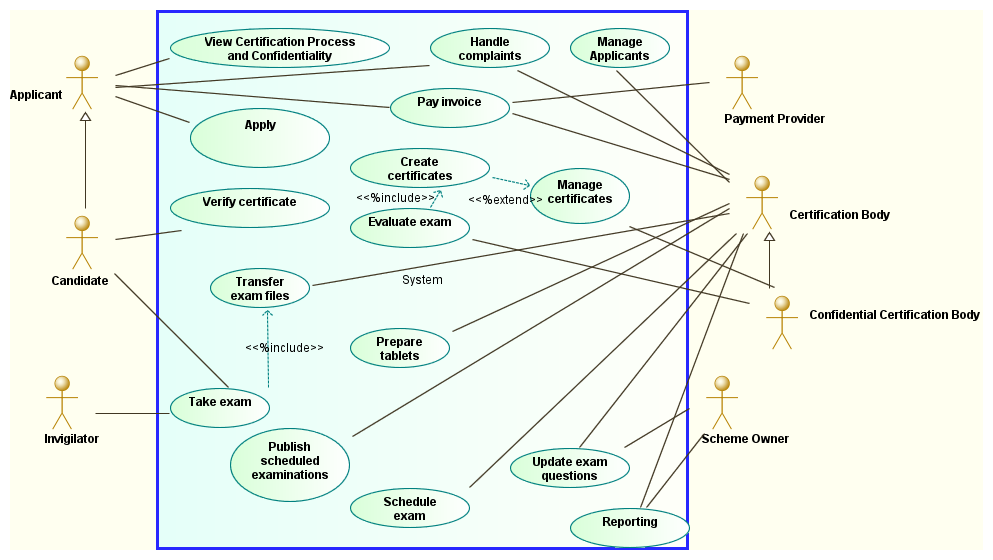
\includegraphics[scale=0.4]{uml/usecase.png}
    \caption{Das mit dem Kunden ermittelte Usecase Diagramm}
\end{figure}

\subsection{Erweiterte Dokumenation der Usecases}
Parallel zur Erstellung des Usecase Diagramms werden zusätzliche Parameter und Beschreibungen für jeden Usecase aufgenommen, welche im eigentlichen Diagramm keine Erwähnung finden.
Dafür wird ein Anforderungstemplate, auch Usecase Beschreibung genannt, verwendet \cite[S. 214]{reqman}, welches aufbauend auf einer Grundversion \cite[Abbildung 8.14, S. 215]{reqman} für jeden Usecase folgende Angaben aufnimmt:

\begin{itemize}
  \item Id: eine eindeutige Bezeichnung, welche dafür verwendet wird, um den Usecase zu referenzieren
  \item Actor: eine Auflistung aller Teilnehmer des Usecases
  \item Description: eine kurze Beschreibung des Usecases
  \item Preconditions: eine Auflistung von Vorbedinungen für den Usecase
  \item Postconditions: eine Auflistung von Nachbedingungen für den Usecase
  \item Normal Course of Events: eine Beschreibung des Standardablaufes
  \item Alternative Courses: Auflistung von Erweiterungen oder zusätzlichen Möglichkeiten
  \item Exceptions: Beschreibung von diversen Ausnahmefälle
  \item Assumptions: Annahmen, unter welcher der Usecase beschrieben wird
  \item Priority: eine Gewichtung, wie wichtig der Usecase ist
  \item Notes: sonstige Anmerkungen
\end{itemize}

Sind die Abläufe komplexer, können Aktivitäts Diagramme verwendet werden, um komplexere Abläufe verständlicher dar zu stellen \cite[S. 215]{reqman}:

\begin{figure}[H]
    \centering
    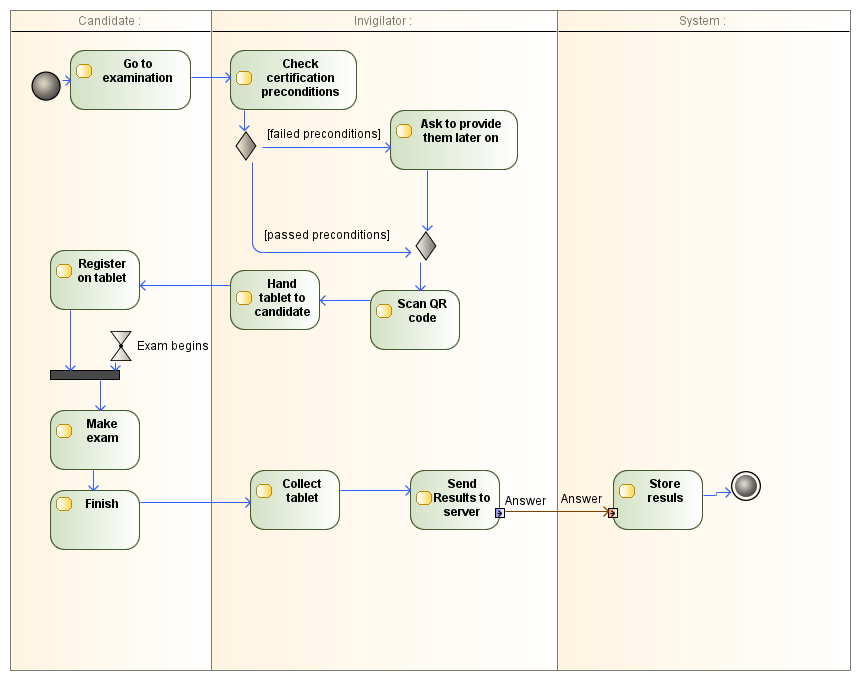
\includegraphics[scale=0.4]{uml/takeexamreq.png}
    \caption{Der Ablauf des Take Exam Usecases im Detail}
\end{figure}

\subsection{Einbeziehen von Architekturreviewparametern}
Um die Einhaltung der Qualitätsparameter zu garantieren, können Architekturreviews durchgeführt werden \cite[S. 20]{review}. Es existiert zwar \glqq keine singuläre, allgemein akzeptierte Metrik um eine Architektur zu beurteilen\grqq \cite[S. 19]{review}, jedoch liefern sie grobe Einschätzungen über die Angemessenheit des Systems \cite[S. 20]{review}. Folgende Architekturreviews wurden dafür ausgewählt:

\begin{itemize}
  \item ATAM: betrachtet Wachstums- und explorative Szenarien um die Architektur zu beurteilen \cite[S. 61]{review}
  \item CBAM: basiert auf ATAM, beachtet jedoch vor allem den Nutzen und die Risiken und Kosten der Architketur, um die Architekturentscheidungen besser abwähgen zu können. Hauptfaktor ist der ROI. \cite[S. 67]{review}
\end{itemize}

Für diese Reviews können bereits früh ein Großteil der benötigten Parameter ermittelt bzw. zumindest grob abgeschätzt werden. Dies ist wichtig, weil nach der 10er Regel der Fehlerkosten früh erkannte Fehler und Probleme weniger Kosten nach sich ziehen als später Erkannte \cite[S. 154]{fehler}.

Deswegen wird das Anforderungstemplate um folgende Parameter erweitert:

\begin{itemize}
  \item Earned Value per month: Wieviel Umsatz der Usecase in einer bestimmten Zeit generiert
  \item Expected Usage: Anzahl der erwarteten Nutzer des Systems pro Zeiteinheit
  \item Growth Scenarios: Anzahl der erwarteten Nutzer des Systems pro Zeiteinheit bei einer höheren Nutzeranzahl
  \item Change Scenarios: mögliche Änderungsszenarien und Erweiterungen
\end{itemize}

\section{Rahmenbedingungen}
Zusätzlich zu funktionalen und nicht funktionalen Anforderungen werden auch die Rahmenbedingungen ermittelt, unter welchem das System erstellt werden soll. Diese Anforderungen beinhalten meist den organisatorischen und zeitlichen Ablauf des Projektes und können auch gewisse Technologien vorschreiben, zB. wenn das System in ein bereits bestehendes System integriert werden soll. \cite[S. 9]{review}\cite[S. 110]{softarch}

Die Rahmenbedingungen des Beispielprojektes lassen sich zum Großteil aus dem ISO Standard für Zertifizierungsstellen ermitteln \cite{ISO_CERT} und geben Einsicht in die Vertraulichkeit der Daten und eröffnen weitere Usecases. Sofern möglich werden diese Parameter in das Usecase Diagramm und das Klassen Diagramm der zu verwendeten Daten mit einbezogen. Auf zeitliche und technologische Rahmenbedingungen wurde im Beispielprojekt nicht eingegangen.

\section{Ermittlung der Daten}
Die zu speichernden Daten werden ermittelt und mit Hilfe eines Klassen Diagrammes modelliert. Dies ist nicht nur wichtig und nützlich, weil die Beispielanwendung in diesem Falle eine stark datenzentrierte Anwendung ist \cite[S. 105]{effektiv}, sondern wird später auch einen wesentlichen Beitrag zur Aufteilung des Systems in Komponenten leisten. Im Falle des Beispielprojekts wurden folgende Daten ermittelt und modelliert:

\begin{figure}[H]
    \centering
    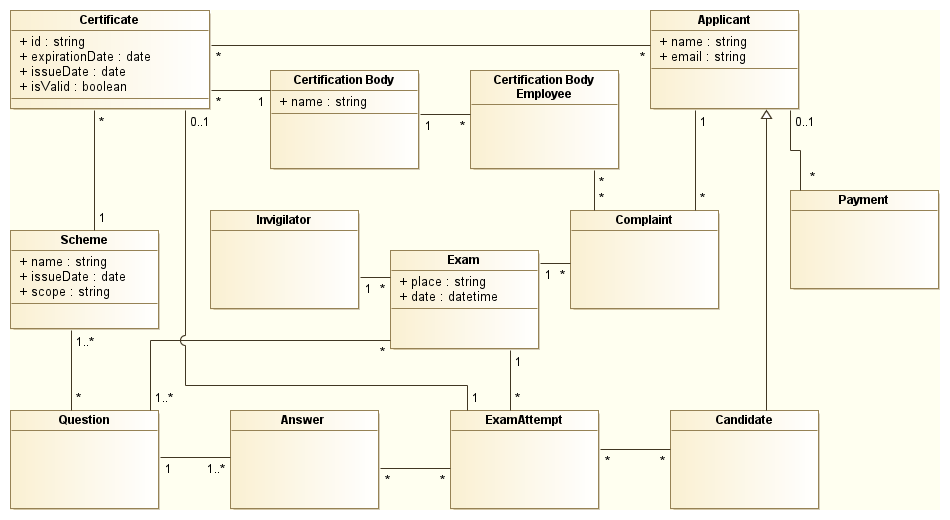
\includegraphics[scale=0.5]{uml/class.png}
    \caption{Das ermittelte Klassendiagramm des Beispielprojektes}
\end{figure}

\section{Datenaufteilung nach Lesendem Zugriff}
Nach der Ermittlung der Daten wird auf Basis der Rahmenbedingungen und Sicherheitsstruktur zusammen mit dem/der Kunden/Kundin ermittelt, welche Daten in welche Vertrautheitskategorien fallen. Dazu werden die Daten anhand ihrer gewollten Lesbarkeit in mehrere Untergruppen unterteilt.

Ermittelt wurden in diesem Falle folgende drei Kategorien:

\begin{itemize}
  \item Public: öffentlich zugängliche Daten, welche auf der Webseite zugänglich gemacht werden
  \item Internal: Daten, welche für die inneren Abläufe Betriebs notwendig sind, aber nicht öffentlich zugänglich sein sollen
  \item Confidential: Daten, welche innerhalb des Betriebes verwendet werden, aber eine besondere Geheimhaltungspflicht und Zugriffschbeschränkung benötigen. Dieses Vertrautheitslevel wurde aufgrund der Rahmenbedingung des Vertraulichen Umgangs mit Prüfungsdaten ermittelt \cite[7.3]{ISO_CERT}
\end{itemize}

Um diese Vertrautheitskategorien besser zu visualisieren zu können wird das UML Metamodel mit Hilfe eines Profiles angepasst. Jede Kategorie erhält einen gleich lautetenden Stereotypen \cite[S. 518]{glasklar}:

\begin{figure}[!htbp]
    \centering
    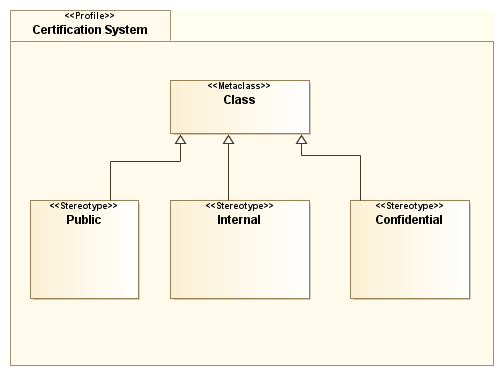
\includegraphics[scale=0.5]{uml/datastereotypes.png}
    \caption{UML wird mit einem Profil um drei Stereotypen erweitert}
\end{figure}

Nach der Erstellung der Stereotypen werden die Daten mit den Vertrautheitskategorien versehen. Sollte es nicht eindeutig sein, welche Klasse in welche Kategorie fällt, müssen die Daten aufgespalten werden und mit einer Assoziation modelliert werden.

\begin{figure}[!htbp]
    \centering
    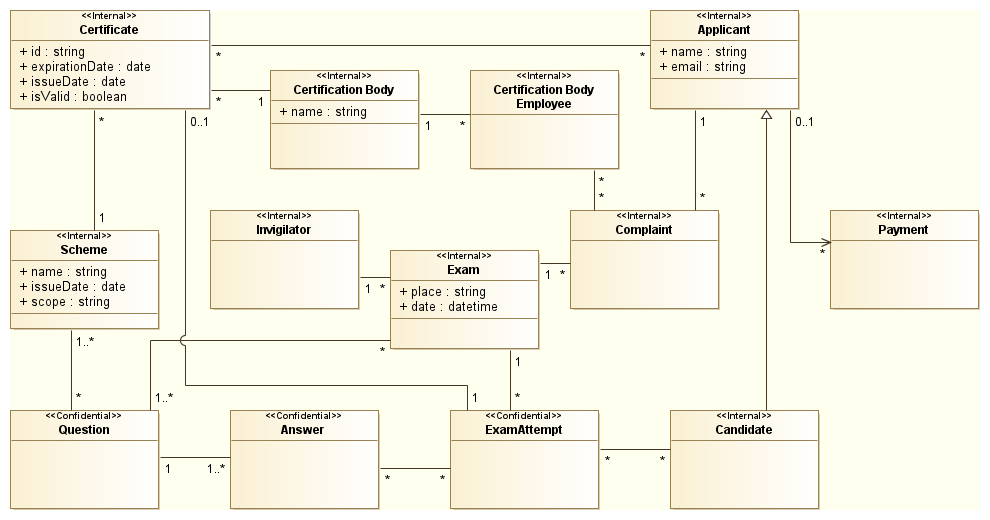
\includegraphics[scale=0.5]{uml/classstereotyped.png}
    \caption{Das Klassendiagramm wird mit Stereotypen der Vertraulichkeit erweitert}
\end{figure}

Überlegung:
* Daten werden in beiden Systemen benötigt:
 * Daten werden im System gespeichert, auf dem Schreibzugriff sein soll
 * System ohne Schreibzugriff synchronisiert diese Daten falls nötig, ansonsten einfach die services aufrufen
 * Auf beiden Systemen schreibzugriff -> bleibt im System

 TODO: vermerken dass das bsp projekt datenzentriert ist, nachschauen ob datenflussarch der richtige begriff ist

wer zugriff auf system mit daten hat kann daten abfangen
Schreibender zugriff?


\section{Modellierung der Akteure und Partnersysteme}
Kontextdiagramm der Akteure und Systeme
